\documentclass[sigconf,review, anonymous]{acmart}
% \documentclass[sigconf,authordraft]{acmart}
% \documentclass[sigconf]{acmart}
\acmConference[ESEC/FSE 2020]{The 28th ACM Joint European Software Engineering Conference and Symposium on the Foundations of Software Engineering}{8 - 13 November, 2020}{Sacramento, California, United States}



% \usepackage{cite}
\usepackage{amsmath,amssymb,amsfonts}
\usepackage{algorithmic}
\usepackage{graphicx}
\usepackage{textcomp}
\usepackage{xcolor}
% \usepackage{hyperref}
\usepackage{tabularx}
\usepackage{multirow}
% \def\BibTeX{{\rm B\kern-.05em{\sc i\kern-.025em b}\kern-.08em
%     T\kern-.1667em\lower.7ex\hbox{E}\kern-.125emX}}

%%
%% \BibTeX command to typeset BibTeX logo in the docs
\AtBeginDocument{%
  \providecommand\BibTeX{{%
    \normalfont B\kern-0.5em{\scshape i\kern-0.25em b}\kern-0.8em\TeX}}}

%% Rights management information.  This information is sent to you
%% when you complete the rights form.  These commands have SAMPLE
%% values in them; it is your responsibility as an author to replace
%% the commands and values with those provided to you when you
%% complete the rights form.
\setcopyright{acmcopyright}
\copyrightyear{2020}
\acmYear{2020}
\acmDOI{10.1145/1122445.1122456}

%% These commands are for a PROCEEDINGS abstract or paper.

\acmBooktitle{ESEC/FSE 2020: ACM Symposium on Neural Gaze Detection,
  June 03--05, 2018, Woodstock, NY}
\acmPrice{15.00}
\acmISBN{978-1-4503-XXXX-X/18/06}





\begin{document}



\title{Hybrid Deep Neural Networks to Infer State Models of Black-Box Systems}

\author{Mohammad Jafar Mashhadi}
\affiliation{%
  \institution{University of Calgary}
%   \streetaddress{P.O. Box 1212}
  \city{Calgary}
  \state{Canada}
%   \postcode{43017-6221}
}
\email{mohammadjafar.mashha@ucalgary.ca}

\author{Hadi Hemmati}
\affiliation{%
  \institution{University of Calgary}
%   \streetaddress{P.O. Box 1212}
  \city{Calgary}
  \state{Canada}
%   \postcode{43017-6221}
}
\email{hadi.hemmati@ucalgary.ca}

\author{Neil Walkinshaw}
\affiliation{%
  \institution{University of Sheffield}
%   \streetaddress{P.O. Box 1212}
  \city{Sheffield}
  \state{UK}
%   \postcode{43017-6221}
}
\email{n.walkinshaw@sheffield.ac.uk}

\begin{CCSXML}
<ccs2012>
   <concept>
       <concept_id>10010147</concept_id>
       <concept_desc>Computing methodologies</concept_desc>
       <concept_significance>500</concept_significance>
       </concept>
   <concept>
       <concept_id>10010147.10010178</concept_id>
       <concept_desc>Computing methodologies~Artificial intelligence</concept_desc>
       <concept_significance>500</concept_significance>
       </concept>
 </ccs2012>
\end{CCSXML}

\ccsdesc[500]{Computing methodologies}
\ccsdesc[500]{Computing methodologies~Artificial intelligence}

\begin{abstract}
What's left:
\begin{itemize}
    \item Abstract
    \item Introduction
    \item Editing `proposed model'
    \item Redrawing the diagram
    \item Experiment sub sections
    \item Results
    \item Discussion
\end{itemize}

\end{abstract}
\keywords{Recurrent Neural Network, Deep Neural Network, Reverse Engineering, Black-box Model Generation}


\maketitle

\section{Introduction}
The contributions of this paper can be summarised as:
\begin{itemize}
    \item Introducing a novel method to infer state models from black-box systems
    \item Proposing a convolutional-recurrent hybrid neural network architecture to extract the hidden internal states just by examining the input-output values of the system. This deep learning model can automatically perform feature extraction making it way more effective and flexible compared to traditional methods. In addition to that we do not make any assumption about statistical properties of the data which makes it applicable to a wider range of problems.
    \item Comparing our proposed method with existing state of the art and state of practice approaches using real world data from a large scale AutoPilot system developed by our industry partner.
    The results show ........ .
    \item Proposing a way to combine change point detection algorithms and EFSM model inference algorithms to infer state models 
\end{itemize}

The rest of the paper is organized as follows: In section blah blah  
\section{Motivation}
Black-box systems are used often in various applications. 
Probably most of the tools and software that we use everyday in our work or every-day life are black-box systems; meaning that we do not have access to their internal workings and their source code and cannot make any changes to them.
But in the end of the day, black box systems just like any other human developed systems are not perfect.
They are prone to have bugs or faults. For that reason, depending on the application, we might need to verify if they work as advertised. For some cases there are standards and authorities that perform the verification on the users' behalf, for example there are FAA certificates for aircraft and street-legality requirements for cars, but this is a luxury not available in all markets. Even on the systems that do have the standards and inspections we might need further more strict and more customized verifications.

Creating a model of the system we have in hand proves to be extremely useful. 
In addition to verification, it can be used for debugging \cite{jafar2019interactive, hybriddebugging, shang2013assisting} and for testing \cite{Walkinshaw2018TestingBlackBox, ModelBasedTesting, Papadopoulos2015, dallmeier2011automatically}.
In this paper we focus on state-based family of systems.


Black-box model inference methods are quite useful when some one decides to use COTS components and they need to inspect the components to verify if work as expected, debug them, or maybe even reverse engineer them. This is a very common scenario in the defense industry.

We propose a method to infer state models from black-box systems which can be put to various uses. An state model helps us to know the internal state of the system which we can use to predict how it will behave in near future.
% This model provides a non-linear approximation of the system
This method helps automate and accelerate model inference therefore facilitating the larger process model inference is a part of. 


What that we test our method on is a commercial UAV\footnote{Unmanned Aerial Vehicle} AutoPilot: a black-box safety critical state-based system. As a black-box its inputs and output signals are accessible. Interpreting them as numerical values id pretty straightforward. However our method is not limited to simple numerical inputs and outputs. 
With some changes it can be used for similar systems such as IoT devices, intelligent video surveillance systems, driver assisting systems, and self driving cars.

\section{Background}
\subsection{State Model Inference}
Roughly speaking, EFSM\footnote{Extended Finite State Machines, are special kind of state machines that have conditional expressions called `transition guards' on their transitions. A state transition can only happen if the transition guard evaluates true.} inference algorithms generally take a list of `events` (along with some variable values) as the input \cite{walkinshaw2016inferring}. They use the events to find the state transitions and the values for detecting invariants and generating guard  conditions for the transitions. 

\subsection{Change Point Detection}
A fundamental tool in time series data analysis is Change Point Detection (CPD). It refers to the task of finding when the model generating the values has changed. 
They can generally be categorized into two main groups: online methods that process the data in real time and offline methods that start processing the data after receiving all the values  \cite{Truong2018ChangePointSurvey}. 
In this paper we only look at offline approaches to stay relevant.


This problem has been tackled from various perspectives. There are hundreds of papers in the literature contributing in this widely used field over the past decades. \cite{chen2011parametric, hasan2014information, hsu1982bayesian, lee2017implicit, oh2002analyzing, ramos2016anomalies, reeves2007review, rosenfield2010change, wang2011non, xie2013sequential, yamanishi2004line, Lavielle1999} Bayesian models focus on finding changes in parameters of underlying distributions generating the data \cite{Lee2018TimeSeriesSegmentation, adams2007bayesian, bai1997estimation, barry1993bayesian, erdman2008fast, ray2002bayesian}. Several methods have used penalty function based methods to find models best fitting each segment of the signals \cite{Lavielle1999, lavielle2005using, keshavarz2018optimal, pein2017heterogeneous}. With a slight change in the penalty function, they are usually usable for detecting known and unknown number of change points. 

Ives and Dakos utilized locally linear models and used statistical significance test to determine at which point the changes in model parameters are large enough to signal a change in the state \cite{Ives2012}. Blythe et al used subspace analysis to reduce data dimensionality to keep the most non-stationary dimensions. This process helps detecting change points more effectively \cite{Blythe2012}. 
%The review: \cite{Truong2018ChangePointSurvey}



\subsection{Deep Learning}
Deep neural networks have shown great 

CNNs

RNNs

Hybrid networks

. DeepSense \cite{deepsense}: Detects the state of mobile user based on sensor input such as accelerometer  \\
. Wearable moltimodal phase \cite{Ordonez2016}\\
. Survey \cite{wang2019deep} 4.6 for CNN-RNN Hybrid related work\\
.. CNN + Dense RNN $>>>$ CNN + Dense \cite{morales2016deep}\\
.. Similar conclusion in \cite{singh2017transforming}\\
.. DRNN outperforms CNNs and DBN (Deep believe networks) \cite{murad2017deep} Also Section 3 presents a background overview of RNNs and LSTM.\\
.. \cite{zheng2016exploiting}\\

\section{Hybrid Neural Network for State Inference}
\textit{I think some of these can be moved over to background/related work section}

In this section we describe our proposed deep learning approach to the state inference task. 
We aimed to infer high level states of a black-box system using a machine learning model that can model the system's behaviour. 

\subsection{Data Format} \label{data_collection}

% To train the model some training data is required. 
To collect data we run the system $N$ times and record the input/output values. The recorded data from each run forms a discrete multi-variate time series data that we show by $T_k$. 
% The set of all $T_k$s is the whole data set $DS$.
% \begin{equation}
%     DS = \{T_k\}_{k=1}^N
% \end{equation}
Multi-variate time series are defined as a set of $n$ univariate time series ($V_i$) of the same length $l_k$. In our case, each $V_i$ is the list of recorded values for one of the inputs/outputs.
\begin{equation}
    T_k = \{{V_1}_k, {V_2}_k, \ldots, {V_n}_k\}
\end{equation}
\begin{equation}
    |{V_1}_k|=|{V_2}_k|=\ldots=|{V_n}_k|=l_k 
\end{equation}


Ideally in each run the system will go through some internal state changes which are labeled manually by a domain expert. In section \ref{mp_data_collection} we explain what we did to keep the variety of the collected data (and hence its quality) high.

The input/output values data are half of the data. We also need a set of true labels to be predicted to complete the data set.
A typical way to obtain the labels is to get some help from domain experts. For each run the y provide a set of tuples in form of $(t_s, s)$ where $t_s$ denotes the timestamp where the system entered state $s$. We show the set of all possible states with $S$ ($s \in S$) and define $N_s$ as the cardinality of this set. 
\begin{equation}\label{eq:change_point}
    CP_k = \big\{ (t_{s_1}, s_1), (t_{s_2}, s_2), \ldots, (t_{s_l}, s_l) \big\} , s_i \in S
\end{equation}
$$N_s = |S|$$


Domain experts know what the system is and what it is supposed to do, so they can (with probably some inherent human error) provide information about the system state. 
they can determine the state from a variety of information sources such as examining the system's I/O (which we have already captured to use for training the model), the logs, or a high level program or set of instructions preloaded into the system.
As the internal workings do not need to be known to perform the labeling, this process does not violate that the system is a black-box.


\begin{figure}[ht]
    \centering
    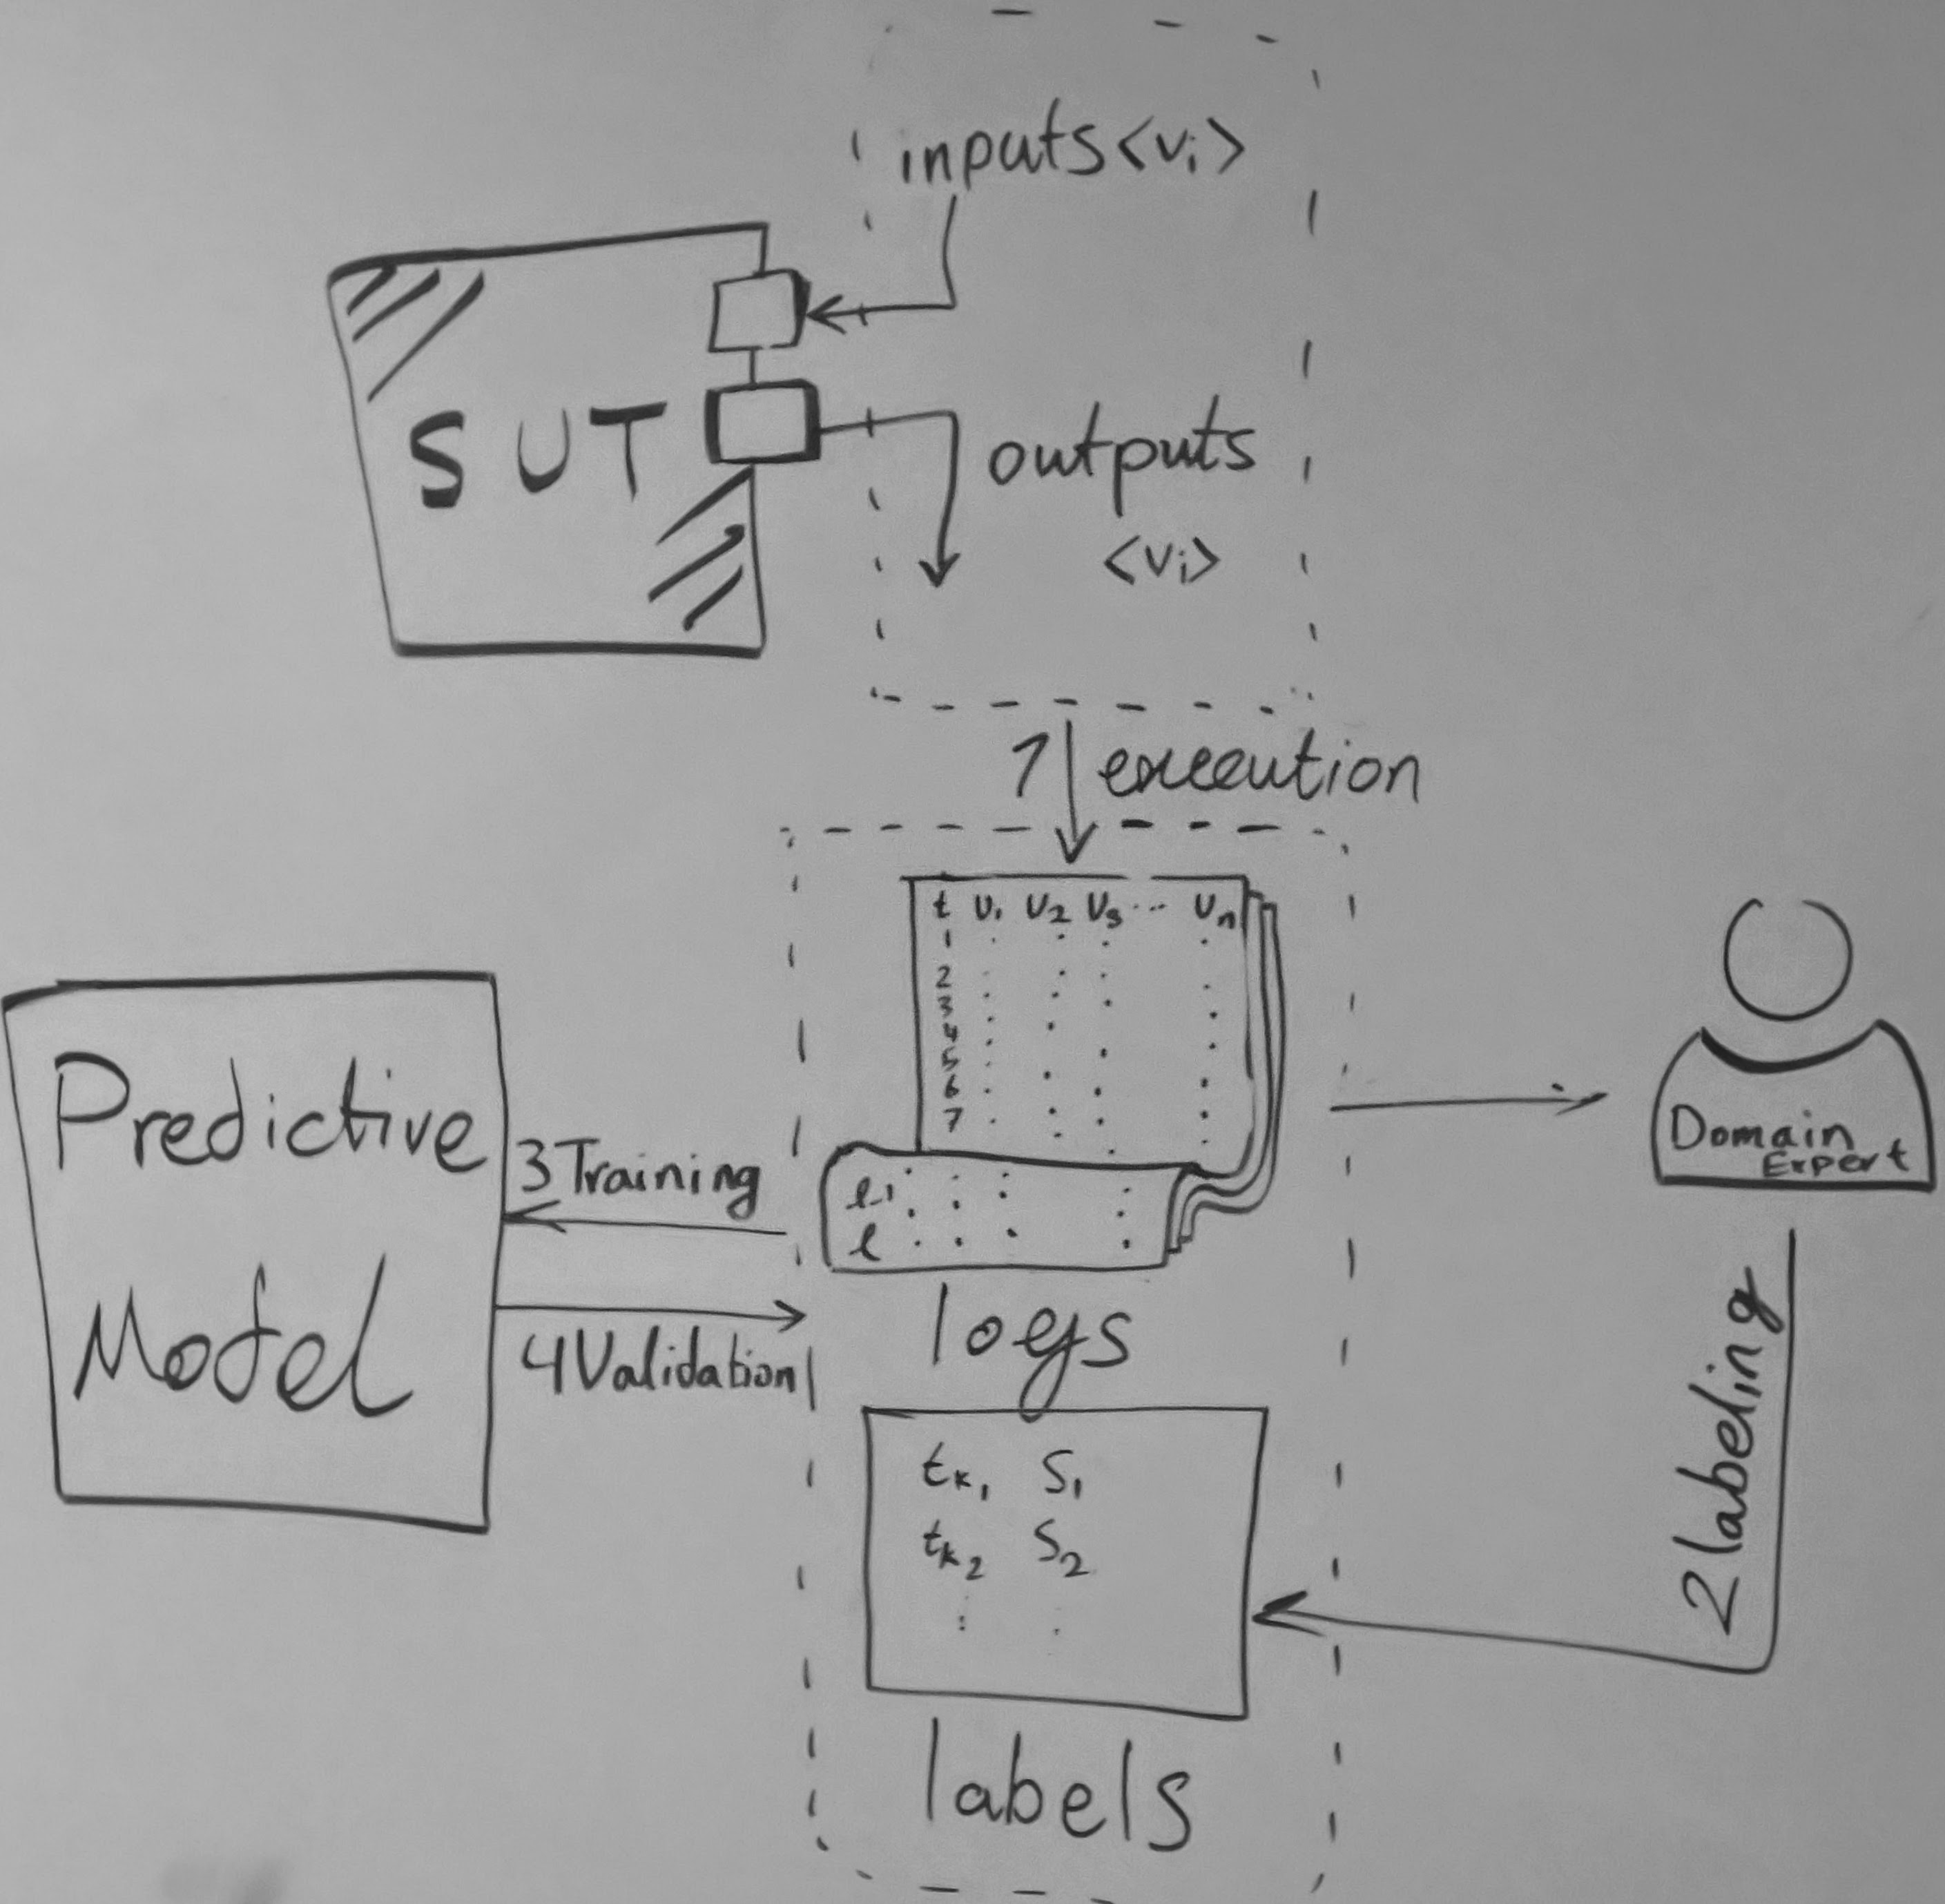
\includegraphics[width=\columnwidth]{Sections/process_diagram.jpg}
    \caption{This diagram shows a big picture of how this technique is applied. The object system is treated as a black-box where we can only read its input and output values. In the first step the system is executed and multiple logs of the input/output values are recorded. Second, a domain expert labels the logs indicating the time stamps where the system's internal state has changed as well as the new state that it went in. In third and fourth steps, as it is typical in machine learning based solutions these data and labels are used for training and validating a machine learning model.}
    \label{fig:process_diagram}
\end{figure}

Combining all, each training instance will be the tuple $(T_k, CP_k)$.

\subsection{Proposed Machine Learning Model}
\subsubsection{Inputs and Labels} \label{data_set_properties}


Since TensorFlow requires all the data to have the same shape, the shorter $T_k$s should be zero-padded to length ,$L = max\{l_k\}$.
Therefore in the end the input to the model will be $T_k$s that are rearranged to form a tensor of shape $n \times L$ along with a padding mask. Padding mask is used to prevent the added zero values having a negative effect on the model's performance. It tells the model where the tail starts so the model can ignore all the zeros from there on.

The true labels ($O$, also called labels in ML literature) is a vector of length $L$ (after padding) where each element $\o_t$ holds the one-hot encoded state at time $t$. It can be determined easily by consulting set $CP_k$ (definition \eqref{eq:change_point}) as defined in \eqref{eq:output}.
\begin{equation} \label{eq:output}
\begin{split}
O = \langle  \forall t \in \mathbb{N}_L : s_i | 
            &{} (t_{s_i}, s_i) \in CP_k \land  \\
            & t_{s_i} = max\{t_{s_j} | (t_{s_j}, s_j) \in CP_k \land t_{s_j}\leq t\} \rangle
\end{split}
\end{equation}
The tensor shapes mentioned here ignore the batch size dimension.

The goal is to find a model $\mathcal{F}(T^p, \mu) \colon \mathbb{R}^{L\times n}\times\mathbb{R}^L\to\mathbb{R}^{L}$ that best approximates the system's behaviour in terms of estimating its internal state given the $n$ time series containing sampled in/out values of the system all zero padded to length $L$.

\begin{equation}\label{eq:model_as_function}
\begin{split}
    \hat{O} = \langle \hat{o}_i \in S \rangle^L_{i=1} {}&{}= \mathcal{F}\left(\left[ {V^p_1}^\intercal \: {V^p_2}^\intercal \; \ldots \; {V^p_n}^\intercal \right], \langle {mask}_j \rangle^L_{j=1}\right) \\
    \langle {mask}_j \rangle^l_{j=1} {}&{}= 1  \\
    \langle {mask}_j \rangle^L_{j=l+1} {}&{}= 0 \\
    V^p_i {}&{}= \left[V_i \quad \vec{0}_{L-l}\right]
\end{split}
\end{equation}

In \eqref{eq:model_as_function} $l$ denotes the length of the input before padding; for the $k$th training data ($T_k$) it is the same as $l_k$. The superscript $p$ for input variables emphasises on the post-padding applied on the original variables which is also shown in the equation.

\subsubsection{Architecture}


We used 4 convolutional layers with 64 filters and kernel sizes of 3, 5, 10, 15 respectively.
%with max pooling layers of size 2 in between. 
Their output is fed into two recurrent layers with 128 and 96 cells each which are then fed into two fully connected layers of size 96 and $N_s$ units. This last layer has a `softmax' activation function.
%This layer's output is fed to an upsampling layer to match the length of the output to length of the labels vector.  
This architecture forms a CNN-RNN hybrid neural network. \cite{Wang2017}


\subsubsection{Architecture Justification}
As mentioned in \ref{changes_in_inputs} since what matters more are the changes rather than the absolute values, applying a derivation operation (or more generally a gradient) is necessary at some point in the processing. 
Farid and Simoncelli enumerated some discrete derivation kernels \cite{Farid2004}, but to have a more generalized notion of discrete derivatives we used convolutional layers in a neural network model. 

Applying convolutional filters on signals is pretty much a standard process in signal processing projects that take deep learning approaches.  \cite{morales2016deep, zeng2014convolutional, yang2015deep} Since convolutional layers on time series basically provide a way to perform calculations on the signal readings spanning a window of time they are effective in capturing features involving temporal relations and invariants in the signals. \cite{wang2017time} 
Using convolutional layers instead of predefined kernels allows the model to learn which subset of possible correlations (which can involve two or more variables) it needs to focus on. This type of flexibility has another benefit as well. It helps the model to be more resilient to time lag between noticing a deviation in input signals and the reaction that will appear in the output signals. This time lag can be caused by a number of reasons including: physical limitations, sampling resolution, tuning of the controller, or design choices in the system.

The recurrent layers introduce an element of `memory' allowing them to capture long-term temporal dependencies which is quite useful in our use case. \cite{Che2018} RNNs have shown promising results in various deep learning for time series tasks such as prediction and classification. \cite{wang2017time, murad2017deep, yang2015deep, Ordonez2016}

This architecture is in part inspired by auto-encoder architectures proposed for image segmentation task. (Add citations and more explanation)
\section{Experiment and Evaluation}
In this section we reiterate the problem, provide more detail about the experiment and evaluation process, and describe the system and the data we collected from it to perform the study.


\subsection{Objectives}
The questions we seek the answer(s) for are as follows:


\textsc{RQ 1) Can existing multivariate time series CPD algorithms be used to detect state changes?}


\textsc{RQ 2) How does our approach compare to similar approaches with classical machine learning algorithms (as opposed to deep learning algorithms)?}


\textsc{RQ 3) How does our approach compare to other algorithms?}


\subsection{Metrics}
% To have a quantitative analysis of the algorithms we measure the following metrics.

Our model combines two tasks, finding when a state transition has happened and finding what the new state is. Traditional state models such as EFSMs do not take time (\textit{when} the transition happens) into account. They focus on finding the right invariants and state transitions (\textit{what} the new state should be).

In time series segmentation literature however, the focus is primarily on answering the \textit{when} question rather than the \textit{what}. Since our model tries to answer both, we need metrics that accommodate both.

In CPD-natured tasks there is an inherent class imbalance.
There are far more points where a change has not happened, so the sheer number of true negatives makes metrics such as accuracy almost useless. 
A trivial model can always output 0 (no change) and have an accuracy of 99\% on a input of length 1000 with 10 true change points.
To address this problem, metrics such as precision and recall that do not account for true negatives are used. \cite{Truong2018ChangePointSurvey, Lee2018TimeSeriesSegmentation} 
Precision and recall for that trivial model will be 0 better reflecting its poor performance.


\subsubsection{Modified F1-Score}
F1-Score the harmonic mean of precision and recall. 
To define precision and recall we need to define true positive, false positive, and false negative first.
Similar to \cite{Lee2018TimeSeriesSegmentation} and \cite{Truong2018ChangePointSurvey}, we use a tolerance margin $\tau$, and if a detected state transition ($\in \hat{CP}_k$) is within $\pm\tau$ of a true transition that is a true positive. 
This tolerance covers the \textit{when}, to take the \textit{what} into the frame we use a parameter $0 \leq \alpha < 1$ that penalizes detecting transitions at a correct time but to an incorrect state.

\begin{equation} \label{eq:cp_hat}
\hat{CP}_k = \big\{(t, \hat{o}_t)\: |\: \hat{o}_t \neq \hat{o}_{t-1} \big\}
\end{equation}

Please note that in \eqref{eq:cp_hat}, $\hat{o}_t$ refers to $t$th element of output vector $\hat{O}$, as previously defined in \eqref{eq:model_as_function}.

\begin{equation}
TP =\sum_{(\hat{t}, \hat{s}_t) \in \hat{CP}_k} \mathcal{TP}(\hat{t}, \hat{s}_t)
\end{equation}
\begin{equation*}
\mathcal{TP}(\hat{t}, \hat{s}_t) =
     \begin{cases}
       1      &\quad \exists\: (t, s_t) \in CP_k \;\text{s.t.}\; |t - \hat{t}| < \tau \land s_t = \hat{s}_t \\
       \alpha &\quad \exists\: (t, s_t) \in CP_k \;\text{s.t.}\; |t - \hat{t}| < \tau \land s_t \neq \hat{s}_t  \\
       0     &\quad\text{otherwise.} \\ 
     \end{cases}
\end{equation*}

Similarly we can define false positive and false negative:

\begin{equation} \label{eq:false_negative}
\begin{split}
FP ={}&{}\Big|\big\{ (\hat{t}, \hat{s}_t) \in \hat{CP}_k \;\big|\; \nexists\: (t, s_t) \in CP_k \;\text{s.t.}\; |t - \hat{t}| < \tau\big\}\Big| \\
FN ={}&{}\Big|\big\{ (t, s_t) \in CP_k \;\big|\; \nexists\: (\hat{t}, \hat{s}_t) \in \hat{CP}_k \;\text{s.t.}\; |t - \hat{t}| < \tau\big\}\Big| 
\end{split}
\end{equation}

\subsubsection{Model Fitting Time}


% \subsubsection{Accuracy}
% \subsubsection{The time tolerance measure in \cite{Lee2018TimeSeriesSegmentation}}


\subsection{Baseline Algorithms}
\subsubsection{CPD algorithms}
A hypothesis is that existing multivariate time series CPD algorithms can be used to solve the problem we are trying to tackle if CPD algorithms would be able to reliably mark the time that state changes happen.
These two steps are our proposed approach of doing that:
1) Applying CPD algorithms to find the time when hidden internal state transitions happen. 
2) Using the state transitions as `events' to form the input of EFSM inference algorithms.

\subsubsection{Classical Machine Learning}
A sliding window of size 10 was rolled over the 10 time series and then flattened to make a vector of size 100 as the input dimensions.


. They performed poorly mainly because they don't have a `memory' as LSTM/GRU neural networks do\\
. The training/prediction performance (time) was not good either ($O(n^4)$)\\


\subsubsection{Deep Learning}

\subsection{Evaluation}


The data was randomly split into two chunks of 95\% and 5\% for training and evaluation.
Adam optimizer \cite{kingma2014adam} was used to optimizer a categorical cross entropy loss function in the training process.

% Training: optimizer, epochs, loss function
% . Comparing the architecture with LSTM/GRU \\
% . Smoothing the input using a rolling window average? good or bad idea?\\
% . Loss function: Binary cross-entropy based on KL-divergence that measures how different two distributions are\\


\subsection{Experiment Environment}
Training and evaluation was done on a single node running Ubuntu 18.04 LTS (Linux 5.3.0) equipped with Intel Core i7-9700K CPU, 32 gigabytes of main memory and 8 gigabytes of GPU memory on a NVIDIA GeForce RTX 2080 graphics card.
The code was written using TensorFlow 2's keras API.



\subsection{System Under Study} \label{mp_data_collection}

Our case study was a real-time controller system, an AutoPilot developed by Winnipeg based Micro Pilot Inc. Micro Pilot is the world-leader in professional UAV AutoPilot which develops both the hardware and the software for 1000+ clients (including NASA, Raytheon, and Northrop Grumman) in 85+ countries during the past 20+ years.

What the AutoPilot does can be summarized as `trying to hold some invariants based on the goal/state of the system'.
Whenever a change in the inputs is detected it makes adjustments to its outputs in order to hold the invariants. 
For example if the AutoPilot is in the `hold altitude' mode, it monitors the altimeter's readings and when it goes out of the acceptable range, proportionate adjustments to the throttle or the nose pitch will be made to get it back to the desired altitude. This is basically how a typical feedback loop controller, such as PID or its variations, work. \cite{feedbacksystemsBook}

% Maybe these two paragraphs can be moved somewhere more appropriate
\label{changes_in_inputs}
To work it backwards we capture the input/outputs over time and examine their correlations, i.e. how changes in one of them results in changes in another. When the state of the system changes these relations may change. So if we can capture what the relations are and when they change we can determine the state in which the system is in. 
Of course pinpointing the exact moment when the changes happen is difficult; It is also impacted by the sampling time resolution so the inferred states and the change points are mere approximations, which by the way can be improved to become more precise.

For example when the autopilot transitions from `hold altitude' state to `descend to X ft' state the goal of the system changes to `descend with a constant sink rate of Y ft/min' until it reaches the desired altitude. It results in change in the set of invariants that the AutoPilot is trying to hold which in turn is reflected in how changes in certain inputs (e.g. altimeter reading) cause the autopilot take actions by making adjustments in certain outputs (e.g. throttle and elevator output). 


% \subsection{Data Set} \label{mp_data_collection}
We ran 948 available tests in a software simulator\footnote{It is developed by MicroPilot Inc and provides a realistic simulation of the aerodynamic  forces on the aircraft, the physical environment irregularities (e.g. unexpected wind gusts), and noises in sensor readings} and collected the flight data. The tests were system tests. They include a flight scenario for various supported aircraft. The scenario goes through different phases in flight such as taking off, cruising, following a path, and landing.
We sampled inputs and outputs values at 5 Hz rate.
It is chosen because the AutoPilot reads the sensor values and performs the calculations required to update its output values at the same rate.
The list of AutoPilot inputs and outputs are shown in table~\ref{tab:in_outs}.


\begin{table}[ht]
    \centering
    \begin{tabularx}{\columnwidth}{lX}
\toprule
\multicolumn{2}{l}{\textbf{Inputs}}                                                                              \\ \midrule
Pitch     & The angle that aircraft's nose makes with the horizon around lateral axis                            \\ 
Roll      & The angle of aircraft's wings make with the horizon around longitudinal axis                         \\ 
Yaw       & The angle of rotation of aircraft around the vertical axis                                           \\ 
Altitude  & AGL\footnotemark Altitude                                                            \\ 
Air speed & Speed of the aircraft relative to the air                                                            \\ 
\midrule
\multicolumn{2}{l}{\textbf{Outputs}}                                                                             \\ 
\midrule
Elevator  & Control surfaces that control the Pitch                                                              \\ 
Aileron   & Control surfaces that control the Roll                                                               \\ 
Rudder    & Control surface that controls the Yaw                                                                \\ 
Throttle  & Controller of engine's power, ranges from 0 to 1                                                     \\ 
Flaps     & Surfaces of back of the wings that provide extra lift at low speeds, usually used during the landing \\ \bottomrule
    \end{tabularx}
    \caption{Recorded inputs and outputs of the AutoPilot. The inputs are sensor readings and the outputs are servo position update commands. All of these 10 sampled values (over time) are used as the inputs of the state prediction model}
    \label{tab:in_outs}
\end{table}
\footnotetext{Above Ground Level}


Out of the 948 flight logs, we omitted 60 of them which were either too short or too long (shorter than 200 samples or longer than 20k samples). Figure~\ref{fig:test_lengths} shows the distribution of the remaining log lengths.

\begin{figure}[h]
    \centering
    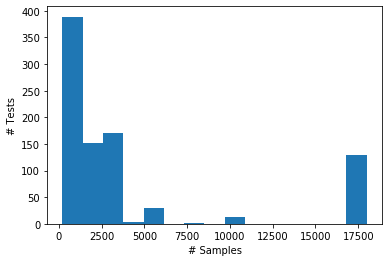
\includegraphics[width=\columnwidth]{Sections/test_lengths.png}
    \caption{Distribution of flight log lengths for the $N=888$ logs that were kept in the data set ($200 \leq l_k \leq 20000$)}
    \label{fig:test_lengths}
\end{figure}

As mentioned in \ref{data_set_properties} each datum is a multivariate time series with $n=10$ variables (listed in table~\ref{tab:in_outs}). 
During the data pre-processing, after the time series data is converted into tensors, all of the shorter $T_i$s were post-padded to the length of the longest one: $L=18001$ time steps. 

\section{Results}
Answers to research questions should come here


Maybe the traditional statistical CPD algorithms could outperform our method if they were boosted by feature engineering. But the feature engineering task is can become an arduous and inefficient task quickly. It exists so it compensates for inability of traditional methods to automatically find meaningful features from the data. \cite{bengio2013deep}



\begin{figure*}[ht]
    \centering
    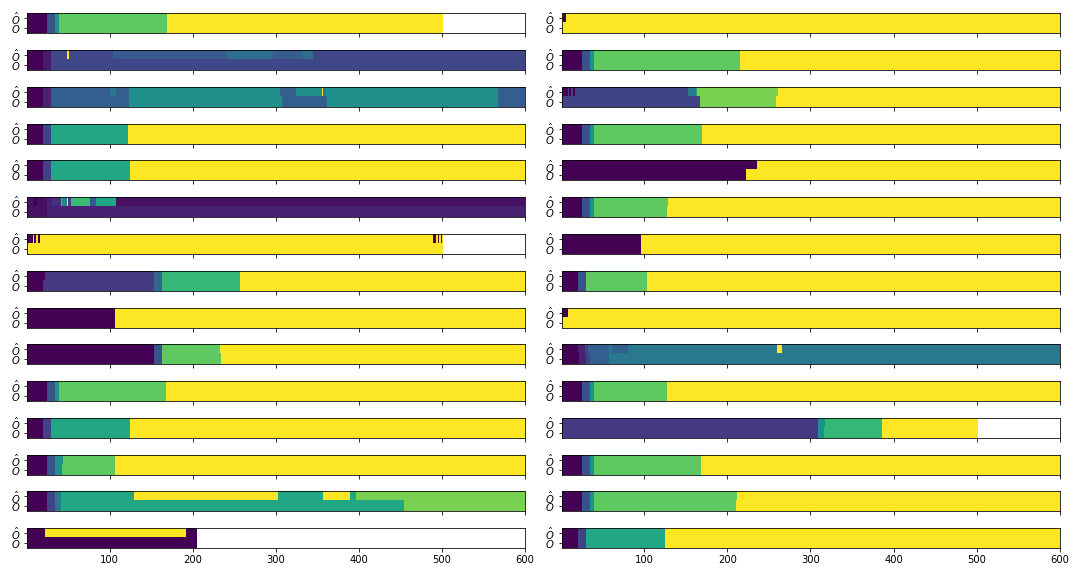
\includegraphics[width=\linewidth]{Sections/test_0.png}
    \caption{Evaluation of the model on unseen data. Each graph shows the state changes in one run of the system. The colors show the states. Top half of each plot depicts model's prediction of the system state ($\hat{O}$) and the bottom half shows the true labels($O$). Since the output is one-hot encoded, the item with the most probability is used as the predicted label at each point in time. X-axis is the time axis. Only the first 600 samples (2 minute of simulation) are shown to improve legibility.}
    \label{fig:test_0}
\end{figure*}
  % and results
\section{Related Work}
% Go paper by paper
. Change point detection using pyramid deep learning model \cite{Ebrahimzadeh2019}\\
. Haidar Khan \cite{Khan2019thesis} Seizure prediction \cite{khan2017focal} -> Section 6.2 has a really good background/related work summary for change point detection \cite{khan2019deep}  \\
. Time series segmentation through automatic feature learning \cite{Lee2018TimeSeriesSegmentation}\\


\section{Limitations and Future Work}
This approach might miss an input-output invariant correlation. It can happen when the input remains constant or it changes too little to reveal its relation with certain outputs. As mentioned in \ref{changes_in_inputs}, this approach relies on changes in signals.

We assume that during the data collection sampling happens in regular intervals; our approach probably will have a hard time achieving high performances processing unevenly spaced time series data.

In this study we saved time and resources by treating a system that we had access to its source code as black-box. Instead of asking a domain expert to label the data, we added some hooks in the code that output the current state. It made the data collection phase much easier, yet one might argue that in practice labeling might get difficult. Albeit on the other hand, having these hooks in the code provided us with too granular state change points which decreases the model's accuracy.

In future endeavours, The possibility and the means of using transfer learning can be studied. Using transfer learning can help reduce the labour intensive task of data labeling. Furthermore, It can enable us to use a pretrained model on similar systems.


\section{Conclusion}


\begin{acks}
% We would like to thank the anonymous reviewers for their constructive comments.
We acknowledge the support of the Natural Sciences and Engineering Research Council of Canada (NSERC), [funding reference number CRDPJ/515254-2017].
\end{acks}

\bibliographystyle{ACM-Reference-Format}
\bibliography{bibilijigili}

\end{document}
\endinput